\documentclass[cameraready]{Interspeech}
\usepackage{float}
\usepackage{amsmath}
\usepackage{hyperref}
\usepackage{graphicx}
\usepackage{tabularx}
\usepackage{array}

\title{Kaggle TensorFlow Speech Recognition Challenge}

\author[affiliation={1}]{Paweł}{Pozorski}
\author[affiliation={1}]{Paweł}{Florek}

\address{
    $^1$ Warsaw University of Technology, Poland
}

\email{\{pawel.pozorski, pawel.florek\}.stud@pw.edu.pl}

\keywords{keyword spotting, Kaggle TensorFlow Speech Recognition Challenge, MLOps, convolutional neural networks, transformers, state-space models, recurrent models}

\begin{document}

\maketitle

\begin{abstract}
Keyword spotting (KWS) serves as the always-on front end of voice interfaces, where low latency and robustness are critical. We present a controlled experimental protocol and MLOps pipeline for comparing KWS architectures on the Kaggle TensorFlow Speech Recognition Challenge dataset. The study design isolates three factors: feature extraction strategy, architectural inductive bias, and non-command handling for \texttt{\_\_unknown\_\_} and \texttt{\_\_silence\_\_}. To ensure fair comparison, all models are trained from scratch under a centralized reproducibility framework with fixed seeds and deterministic controls. Final test evaluation is defined to operate only on Phase 4-selected systems, including single models and within-method ensembles across the three top Phase 3 backbones. This manuscript version documents the protocol and validation plan; empirical performance outcomes are intentionally deferred to a results-complete version.
\end{abstract}

\section{Introduction and Motivation}
Detecting a fixed, limited vocabulary within an audio stream occupies a unique and highly resource-constrained niche in modern speech processing \cite{sainath2015cnn, zhang2017hello}. Recent progress has diversified the model landscape, but many comparisons still confound architectural differences with inconsistent preprocessing and optimization choices. Our objective is to evaluate architectures under a common, from-scratch training protocol, ensuring that observed differences are attributable to structural inductive biases rather than transfer-learning advantages \cite{gong2021ast}.

Our study is structured around three primary research questions, designed to systematically isolate the drivers of KWS efficacy:
\begin{itemize}
    \item \textbf{Q1 (Feature strategy):} Which feature extraction pipeline produces the most generalizable representations for a fixed 1-second classification task? This evaluates whether the default reliance on standard log-mel spectrograms is genuinely optimal.
    \item \textbf{Q2 (Architectural inductive bias):} Which structural prior best captures the temporal-spectral dynamics of brief KWS inputs? We directly compare local spatial hierarchies, global all-to-all attention, and finite-memory sequential compression.
    \item \textbf{Q3 (Non-command class methodology):} Which methodology best recognizes \texttt{\_\_unknown\_\_} and \texttt{\_\_silence\_\_} while preserving macro-F1 on the core command classes?
\end{itemize}

To prevent hyperparameter explosion and to contextualize model evaluation within a practical engineering framework, we structure our experiments into a strict four-phase pipeline (introduced in Section~\ref{sec:phases}). In this manuscript version, the emphasis is methodological: the Results section specifies the held-out test protocol, while empirical comparisons are reported after all runs complete.

\section{Dataset and Task Formulation}
\label{sec:dataset}
To provide a genuine evaluation of raw architectural capacity, this project leverages the Kaggle TensorFlow Speech Recognition Challenge dataset (derived from Google Speech Commands v1) \cite{warden2018speech} as an uncompromising test bed. These constraints eliminate substantial domain-level complexities that typically confound architectural comparisons.

% TODO: Check it
While the canonical Speech Commands v0.01 release is designed to contain uniform one-second samples at $16$ kHz, we observe that the Kaggle variant exhibits distinct deviations: approximately $89.8\%$ of samples are exactly one second, but outliers range from $0.37$ to $95.18$ seconds. The full taxonomy contains $32$ classes in total ($30$ command labels, plus \texttt{\_\_unknown\_\_} and \texttt{\_\_silence\_\_}). Models must therefore be formulated to robustly handle transient temporal padding while strictly discriminating across a multi-class landscape.

\subsection{Unknown-Class Synthesis Methodology}
For the extended dataset configuration, we generate additional \texttt{\_\_unknown\_\_} examples directly from the training corpus without external models. Candidate source clips are drawn from command classes only (excluding \texttt{\_\_unknown\_\_} and background-noise folders), with the hard constraint that clips within one synthetic sample must come from different classes.

Each synthetic item is formed by blending $2$ or $3$ one-second clips. Before mixing, each source is mean-centered, RMS-normalized toward a shared target level, and lightly smoothed with a short delayed component to reduce abrupt local transients. The final mixture is then produced by dense short-frame overlap where all sources remain active throughout the full second with slowly varying weights, encouraging spectro-temporal continuity rather than hard segment boundaries.

To avoid regenerating the same example, uniqueness is tracked at the source-file level (sorted source path tuple), not at the class-combination level. After synthesis, each candidate is passed through an envelope-based smoothness gate (windowed RMS trajectory checks for abrupt jumps and deep internal valleys). If a candidate fails this gate, it is discarded and regenerated in a retry loop; only accepted candidates are written to the \texttt{\_\_unknown\_\_} directory.


% TODO: Insert a visual of the class distribution in the training set, highlighting the dominance of the \texttt{\_\_unknown\_\_} class.
% TODO: Insert EDA visualizations of the raw audio waveforms, showing the diversity of temporal patterns across different command words. Keep entire section under 1.5 pages.

\section{Experimental Design and MLOps Pipeline}
\label{sec:phases}
To systematically address our research questions without combinatorial explosion, we filter configurations through a gated, four-phase funnel. Each phase selects the optimal setup based on macro-F1 across three fixed random seeds, locking that configuration for the next stage. Table~\ref{tab:model_calls} outlines the experiment scope and compute budget.
Due to hardware limitations, all experiments in Phases $1$--$3$ are executed on \texttt{train\_small} and \texttt{valid\_small} (Refer to Section~\ref{sec:dataset} for exact definitions).

\begin{table}[htbp]
\centering
\caption{Estimated Model Training Calls per Experimental Phase.}
\label{tab:model_calls}
\small
\begin{tabular}{@{} p{0.7cm} p{3.5cm} >{\centering\arraybackslash}p{0.8cm} >{\centering\arraybackslash}p{0.5cm} >{\centering\arraybackslash}p{0.8cm} @{}}
\toprule
\textbf{Phase} & \textbf{Experiment Scope} & \textbf{Configs} & \textbf{Seeds} & \textbf{Total Runs} \\ \midrule
\textbf{1} & Feature Strategy Ablation \newline (5 features $\times$ 2 proxy models) & 10 & 3 & 30 \\
\textbf{2} & Global Hyperparameter Tuning \newline (best feature $\times$ 2 proxies $\times$ 4 optim. combos) & 8 & 3 & 24 \\
\textbf{3} & Inductive Bias Comparison \newline (AST: 8, ConvNeXt: 2, SSAMBA: 8, xLSTM: 8, MLP-Mixer: 4) & 30 & 3 & 90 \\
\textbf{4} & Non-Command Method Comparison \newline (5 strategies $\times$ 3 top models on \texttt{\_\_unknown\_\_}/\texttt{\_\_silence\_\_}) & 15 & 3 & 45 \\ \midrule
\textbf{Total} & \textbf{Cumulative Training Executions} & \textbf{63} & & \textbf{189} \\ \bottomrule
\end{tabular}
\end{table}

\subsection{Phase 1: Feature Extraction Strategy (Q1)}
Raw audio waveforms are highly inefficient for direct neural network processing due to a lack of semantic meaning at the sample level and high adjacent correlation \cite{purwins2019deep}. We transform the signal into time-frequency representations using the Short-Time Fourier Transform (STFT) \cite{allen1977short}.

% TODO: Insert visualization of the audio feature extraction pipeline (Waveform -> STFT windowing -> Mel Filterbank -> Log/PCEN Compression).

This extraction is governed by the time-frequency uncertainty principle (Gabor limit), bounding resolution such that $\Delta t \cdot \Delta f \geq \frac{1}{4\pi}$. We encapsulate all preprocessing pipelines within PyTorch \texttt{nn.Module}s to ensure differentiable, GPU-accelerated computations, evaluating five distinct strategies:

\begin{description}
    \item[Mel-Spectrogram (Baseline):] Emulating human auditory non-linearity via the Mel scale ($m = 2595 \log_{10}(1 + f/700)$) \cite{stevens1937mel}, this baseline uses $n_{fft} = 1024$ ($64$ ms window) and a $10$ ms stride. Power spectra are filtered and compressed via an $80$ dB-bounded log-amplitude transform to stabilize gradients.
    \item[High Temporal Resolution Mel:] Shifting the Gabor limit temporally, this setup halves the window and hop sizes ($32$ ms window; $5$ ms stride). The $200$ Hz frame rate exposes sub-phonemic transients otherwise smeared by wider windows.
    \item[MFCC:] Applying a Discrete Cosine Transform (DCT) to log-mel energies projects the signal into the quefrency domain. Retaining $40$ coefficients decorrelates channels \cite{davis1980mfcc} and slashes the data footprint by $\sim93\%$.
    \item[PCEN:] Per-Channel Energy Normalization \cite{wang2017pcen} applies dynamic automatic gain control. It suppresses stationary noise and emphasizes transients \cite{lostanlen2019pcen}, enhancing robustness against varied SNRs.
    \item[Mel + SpecAugment:] Acting as structured input dropout, SpecAugment \cite{park2019specaugment} applies stochastic rectangular masks across time and frequency axes, forcing the model to learn distributed phonetic representations.
\end{description}

To prevent favoring a specific architecture during this phase, we evaluate the pipelines on two proxy baselines: a spatial ConvNeXt model and a sequential xLSTM model. This ensures we do not inadvertently handicap sequential models that might uniquely benefit from high-temporal strides. Table~\ref{tab:feature_strategies} and Figure~\ref{fig:example_features} detail these setups.

\begin{table*}[htbp]
\centering
\caption{Feature extraction strategies compared in Phase $1$.}
\label{tab:feature_strategies}
\scriptsize
\begingroup\setlength{\tabcolsep}{4pt}
\begin{tabularx}{0.8\textwidth}{@{} l c c c c c c c X@{}}
\toprule
Strategy & n\_fft & hop\_length & Window & Hop & Frames & Bins & Approx. input size (1 s) & Augmentation \\
\midrule
Mel (baseline) & 1024 & 160 & 64 ms & 10 ms & 101 & 128 mels & $12{,}928$ ($128\times101$) & none \\
Mel (hi-temporal) & 512 & 80 & 32 ms & 5 ms & 201 & 128 mels & $25{,}728$ ($128\times201$) & none \\
MFCC & 1024 & 160 & 64 ms & 10 ms & 101 & 40 MFCCs & $4{,}040$ ($40\times101$) & none \\
PCEN & 1024 & 160 & 64 ms & 10 ms & 101 & 128 mels & $12{,}928$ ($128\times101$) & none \\
Mel + SpecAugment & 1024 & 160 & 64 ms & 10 ms & 101 & 128 mels & $12{,}928$ ($128\times101$) & freq+time masking \\
\bottomrule
\end{tabularx}
\endgroup
\end{table*}

% TODO: replace it with our custom example, add here also other methods row by row and move this image below the description.
\begin{figure}[htbp]
\centering
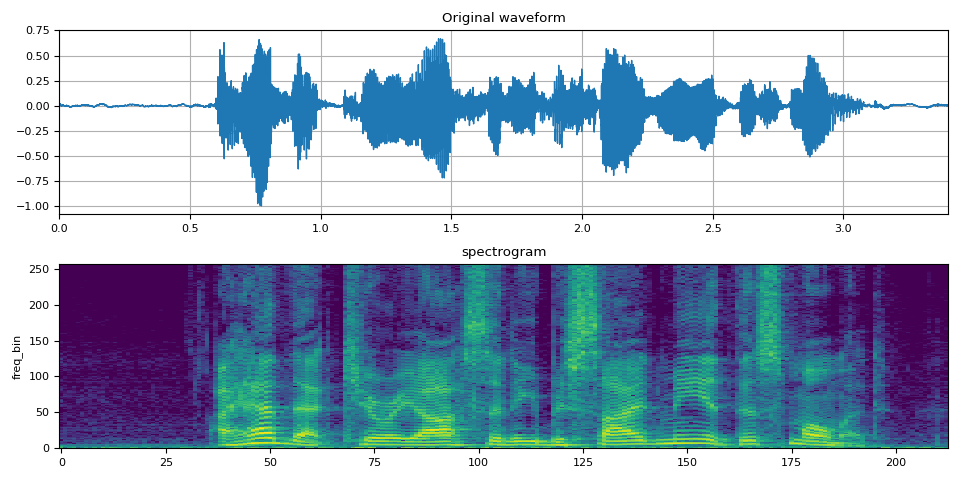
\includegraphics[width=0.95\linewidth]{figures/pytorch_melspec_nfft512.png}
\caption{Top: original waveform. After it, row by row: Mel-Spectrogram, High Temporal Resolution Mel, MFCC, PCEN, and Mel + SpecAugment.}
\label{fig:example_features}
\end{figure}

\subsection{Phases 2 \& 3: Architectural Bias and Optimization (Q2)}
To isolate structural effects, we train all models entirely from random initialization. Rather than asking which pre-training source transfers best, this design asks which architecture inherently learns most effectively from the supervision signal.

Phase 2 locks the global optimization strategy (Table~\ref{tab:global_hyperparams}) using the optimal Phase 1 feature set. Phase 3 then sweeps model-specific hyperparameters (Table~\ref{tab:model_hyperparams}) across five distinct families:

% TODO: Add visual comparison of the structural paradigms: Local spatial (ConvNeXt) vs. Global attention (AST) vs. Sequential state tracking (SSAMBA/xLSTM).

\begin{description}
    \item[AST (Audio Spectrogram Transformer):] Replaces convolutions with self-attention \cite{vaswani2017attention, gong2021ast}, granting a global receptive field from the first layer and assuming all-to-all interactions are necessary.
    \item[ConvNeXt (Modern CNN):] Relies on translation equivariance and local correlation \cite{lecun1995convolutional}. It modernizes residual networks with Vision Transformer elements, testing if local spatial hierarchies remain optimal \cite{liu2022convnet}.
    \item[SSAMBA (Selective State Space):] Adapts Mamba \cite{gu2023mamba} to audio \cite{shams2024ssamba}. By mapping 1D sequences via discretized differential equations, it achieves content-aware focus with RNN-like $O(L)$ efficiency.
    \item[xLSTM (High-Capacity Recurrence):] Solves classical LSTM scalar bottlenecks by introducing matrix memory $C_t \in \mathbb{R}^{d \times d}$ \cite{beck2024xlstm}, providing a pristine test of sequential tracking suitability.
    \item[MLP-Mixer:] Serves as an architectural null hypothesis \cite{tolstikhin2021mlpmixer}, applying alternating dense matrix multiplications without spatial or sequential priors.
\end{description}

\begin{table}[htbp]
\centering
\caption{Global optimization hyperparameters (Phase $2$).}
\label{tab:global_hyperparams}
\small
\begin{tabularx}{\columnwidth}{@{}l @{}>{\centering\arraybackslash}p{2.8cm} X@{}}
\toprule
\textbf{Parameter} & \textbf{Values} & \textbf{Purpose} \\ \midrule
Weight decay & $10^{-2}, 10^{-1}$ & Prevents overwriting of learned features \\
LR scheduler & Cosine Annealing with Warmup / Reduce LR on Plateau & Cosine annealing with linear warmup; or metric-driven reduction \\
\bottomrule
\end{tabularx}
\end{table}

\begin{table}[htbp]
\centering
\caption{Model-specific hyperparameter sweeps (Phase $3$).}
\label{tab:model_hyperparams}
\small
\begin{tabularx}{\columnwidth}{@{}l X@{}}
\toprule
\textbf{Model} & \textbf{Sweep Space} \\ \midrule
\textbf{AST} & Dropout $\{0.1, 0.5\}$; Head \{linear, MLP(256)\}; Pos. Emb. \{interp., learned\} \cite{gong2021ast} \\
\textbf{ConvNeXt} & Stoch. Depth $\{0.0, 0.2\}$; Kernel size $\{7\times7\}$ \cite{liu2022convnet} \\
\textbf{SSAMBA} & Pooling \{mean, max\}; CLS \{yes, no\}; Stride $\{10\text{ms}, 5\text{ms}\}$ \cite{gu2023mamba,shams2024ssamba} \\
\textbf{xLSTM} & Dim $d \in \{32, 64\}$; State Reset \{T, F\}; Output \{final, mean\} \cite{beck2024xlstm} \\
\textbf{MLP-Mixer} & Dropout $\{0.0, 0.2\}$; Head L2 Norm \{yes, no\} \cite{tolstikhin2021mlpmixer} \\ \bottomrule
\end{tabularx}
\end{table}

\subsection{Phase 4: Non-Command Class Methodology (Q3)}
All core models are optimized natively via standard \texttt{CrossEntropyLoss} \cite{goodfellow2016deep}. We intentionally defer imbalance-specific loss shaping and resampling in earlier phases to keep architectural comparisons interpretable. In Phase 4, we freeze the top three architectures from Phase 3 and vary only the non-command strategy, explicitly testing five alternatives for handling \texttt{\_\_unknown\_\_} and \texttt{\_\_silence\_\_}:

\begin{enumerate}
    \item \textbf{Flat multiclass baseline:} unchanged single-head classification over all classes.
    \item \textbf{Sampling control:} weighted random sampling with replacement and fixed target class priors: $p_{\mathrm{unknown}}=0.25$, $p_{\mathrm{silence}}=0.15$, and $p_{\mathrm{cmd},k}=0.02$ for each of the $30$ command labels (summing to $1.0$).
    \item \textbf{Loss reweighting:} weighted cross-entropy with elevated penalties on non-command misclassification.
    \item \textbf{Two-stage detector:} a separate binary gate (command vs. non-command), followed by command-word classification only when the gate predicts command.
    \item \textbf{Shared two-head model:} a command head (30 labels) plus a dedicated non-command head (silence vs. unknown).
\end{enumerate}

For sampling control, if class $c$ has $n_c$ training examples, each example from that class receives weight
$$
w_c = \frac{p_c}{n_c}.
$$
Each epoch draws $N$ samples (with replacement), where $N$ equals the original training-split size. This yields explicit undersampling of \texttt{\_\_unknown\_\_} whenever its empirical share exceeds $25\%$, and oversampling of \texttt{\_\_silence\_\_} and underrepresented command classes to match the target priors above.

To keep comparisons fair, all methods reuse identical data splits and three fixed seeds ($0$, $42$, $2003$). Model selection follows a strict gate: any method that degrades core-command macro-F1 by more than $\delta=1.0$ percentage point relative to its frozen Phase 3 baseline is rejected. Among remaining candidates, we maximize non-command macro-F1,
$$
\mathrm{Macro\text{-}F1}_{\mathrm{NC}} = \frac{\mathrm{F1}_{\mathrm{unknown}} + \mathrm{F1}_{\mathrm{silence}}}{2},
$$
and use silence false-trigger rate and unknown-to-command leakage as tie-breakers.

The outputs of Phase 4 define the final deployable systems and are the only systems advanced to held-out test-set validation. We evaluate three inference flows: (i) single-stage multiclass flow (input $\rightarrow$ one model $\rightarrow$ class), (ii) two-stage detector flow (input $\rightarrow$ binary gate $\rightarrow$ either non-command label or command classifier), and (iii) shared-backbone two-head flow (input $\rightarrow$ shared encoder $\rightarrow$ command head and non-command head, with a fixed decision rule).

\section{Strict Reproducibility and Training Control}
To account for hardware-level non-determinism during GPU acceleration, we execute every experiment three separate times using fixed starting points (seeds $0$, $42$, and $2003$) and report aggregated results (mean $\pm$ standard deviation).

All experiments are run on a single Apple MacBook Pro with an M4 Pro chip, $48$ GB unified memory, and a $512$ GB SSD. This hardware budget motivates the use of \texttt{train\_small} and \texttt{valid\_small} in Phases $1$--$3$.

To reduce sampling bias introduced by subsampling, \texttt{train\_small} and \texttt{valid\_small} are constructed to preserve the label distribution $p(y)$ of their corresponding full splits (stratified downsampling).

We employ AdamW \cite{loshchilov2019adamw} to explicitly decouple weight decay from adaptive gradient scaling, and rely on Kaiming normal initialization \cite{he2015delving}. To guarantee that experiments can be perfectly duplicated, we enforce deterministic data loading and automatically generate a \texttt{ReproducibilityReport} via MLflow \cite{zaharia2018accelerating} for every run. This report logs all environmental conditions, library versions, and the precise state of the codebase.

\section{Results}
Final test reporting is restricted to systems selected in Phase 4, since this stage determines deployment-relevant behavior for \texttt{\_\_unknown\_\_} and \texttt{\_\_silence\_\_}. After model selection on the validation split, each selected system is evaluated once on the held-out test set. We report per-class precision, recall, and F1, together with command macro-F1 and non-command macro-F1.

Beyond single-model results, we evaluate all ensemble combinations across the three Phase 3-derived backbones within each fixed Phase 4 method. Denoting the model outputs by $M_1, M_2, M_3$, we test all non-empty subsets (i.e., $2^3 - 1 = 7$ combinations) and aggregate class probabilities by simple averaging under the same within-method calibration rule. Cross-method ensembles are not considered; every ensemble is built from models produced by one common Phase 4 strategy. These ensemble checks are inference-only and are therefore excluded from the cumulative training execution counts in Table~\ref{tab:model_calls}.

\section{Conclusion}
This work defines a reproducible, four-phase methodology for studying KWS under controlled conditions, from feature selection and architecture comparison to explicit non-command handling. The final systems are those selected in Phase 4, and the evaluation plan includes both single-model testing and within-method ensemble testing across the three best Phase 3 backbones. At this stage, the paper serves as a protocol and analysis blueprint rather than a source of empirical claims. Quantitative conclusions about architecture quality and boundary-class behavior will be drawn only after the full Phase 4 selection and held-out test evaluation are completed.

\bibliographystyle{IEEEtran}
\bibliography{mybib}

\end{document}
